\chapter{Evaluierung}%

\label{cha:Eval}

In diesem Kapitel wird der implementierte Reinforcement-Learning-Agent evaluiert. Hierfür wird zuerst, mit Hilfe von einem deterministischen Gegner und einem Gegner, der in jedem Zug eine zufällige Aktion auswählt, gezeigt, ob die neu gewählte Reward-Funktion einen Vorteil beim Lernen darstellt. Danach wird an diesen beiden Gegnern gezeigt, ob das Lernen mit Einbezug der gegnerischen Züge eine Veränderung im Lernverhalten aufweist. Dann wird gegen den Minimax Algorithmus trainiert, um zu zeigen, wie gut der Reinforcement-Learning-Agent werden kann. \\Es folgen nun die Graphen dieser Evaluierung, wobei immer die zwei nebeneinander stehenden Graphen die selbe Lernepoche beschreiben. Der erste Graph (a,c,e oder g) beschreibt den absoluten Reward, also den genauen Wert zu jeder Episode. Der zweite Graph (b,d,f oder h) beschreibt den durchschnittlichen Reward zu jeder Episode im Bezug auf alle vorherigen Episoden dieser Epoche.
Es wurde sich für eine Epoche von 1000 Episoden entschieden, da sich hier schon das Verhalten des Agenten abzeichnet und das Berechnen von längeren Epochen einen sehr hohen Zeitaufwand bedeuten würde.\\

Es sei darauf hingewiesen, dass der durchschnittliche Reward (b,d,f oder h) meist nicht das komplette Spektrum von 1 bis -1 abdeckt. Dies wurde gemacht um eine bessere Erkennbarkeit des Ausschnittes zu gewähren.

\section{Reward-Funktion}
Als erstes wird die Veränderung durch die zugabhängige Reward-Funktion evaluiert. Hierfür wird Abbildung \ref{fig:randomFF} mit Abbildung \ref{fig:randomTF} sowie Abbildung \ref{fig:leftiFF} mit Abbildung \ref{fig:leftiTF} verglichen.\\
Abbildung \ref{fig:randomFF} (b) und Abbildung \ref{fig:randomTF} (b) verhalten sich fundamental sehr ähnlich. Beide erreichen einen durchschnittlichen Reward von 0.5 nach etwa 250 Episoden wobei die einfache Reward-Funktion aber einen abfallenden, und die zugabhängige Reward-Funktion einen konstanteren Trend aufweist.\\

\begin{figure}%
    \centering
    \subfloat[absoluter Reward]{{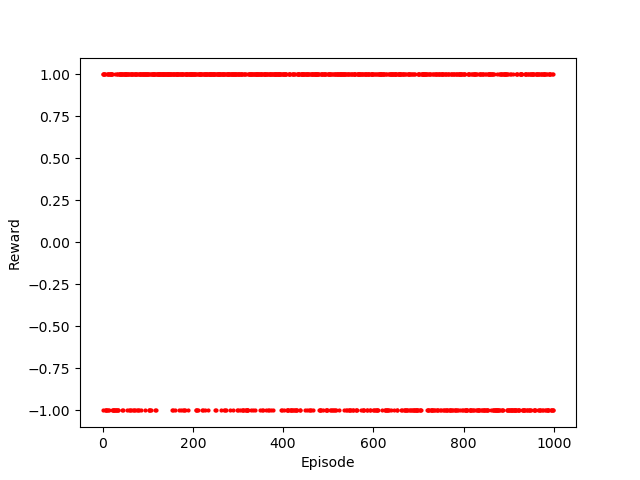
\includegraphics[width=6cm]{RandomFFallreward_plot.png} }}%
    \qquad
    \subfloat[durchschnittlicher Reward]{{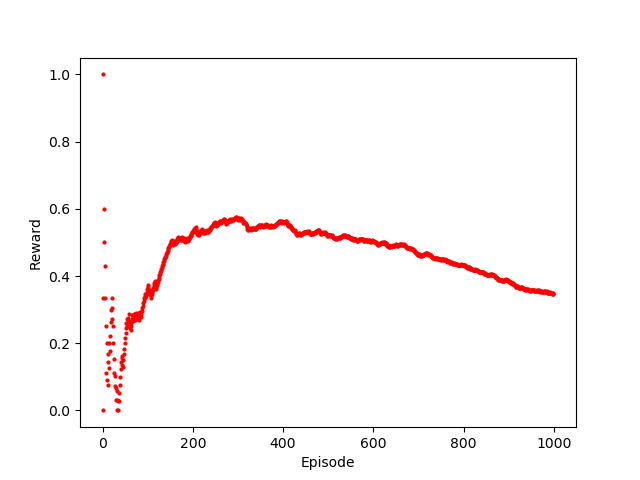
\includegraphics[width=6cm]{RandomFFaveragereward_plot.png} }}%
    \caption{Reinforcement-Learning an zufällig ziehendem Gegner mit einfacher Reward-Funktion und ohne die Züge des Gegners mitzulernen.}%
    \label{fig:randomFF}%
\end{figure}


\begin{figure}%
    \centering
    \subfloat[absoluter Reward]{{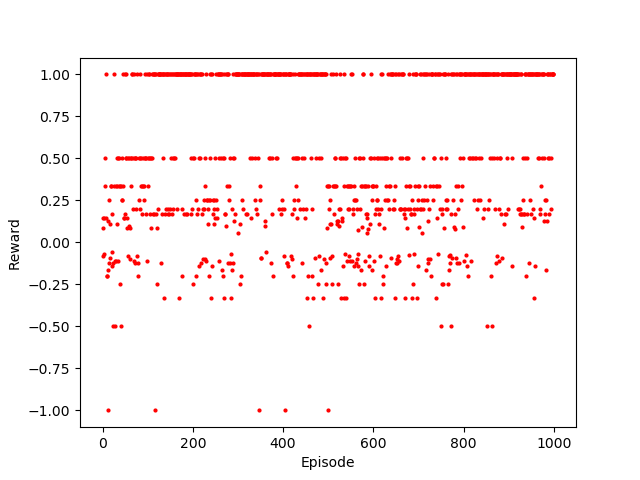
\includegraphics[width=6cm]{RandomTFallreward_plot.png} }}%
    \qquad
    \subfloat[durchschnittlicher Reward]{{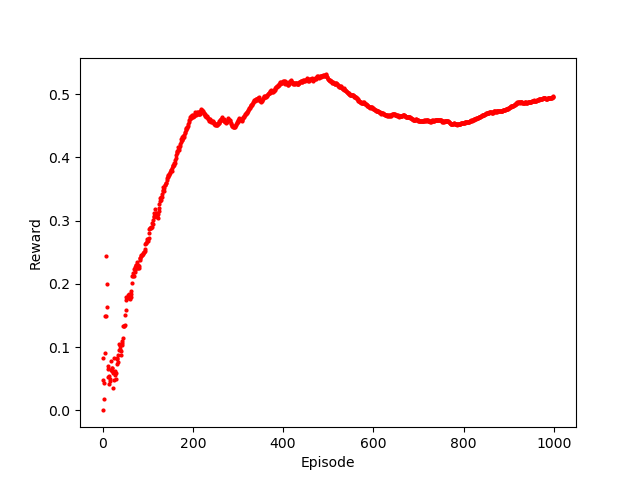
\includegraphics[width=6cm]{RandomTFaveragereward_plot.png} }}%
    \caption{Reinforcement-Learning an zufällig ziehendem Gegner mit verbesserter Reward-Funktion und ohne die Züge des Gegners mitzulernen.}%
    \label{fig:randomTF}%
\end{figure}

Abbildung \ref{fig:leftiFF}(b) zeigt einen starken Abfall in gewonnenen Spielen nach etwa der 300. Episode. Dieses Verhalten ist ebenfalls sehr stark in Abbildung \ref{fig:leftiFF}(a) zu erkennen.\\
Im Vergleich zu der einfachen Reward-Funktion wird in Abbildung \ref{fig:leftiTF}(b) eine Annäherung an 0 aufzeigt, was auf eine 50\% Gewinnchance hinweist.\\

\begin{figure}%
    \centering
    \subfloat[absoluter Reward]{{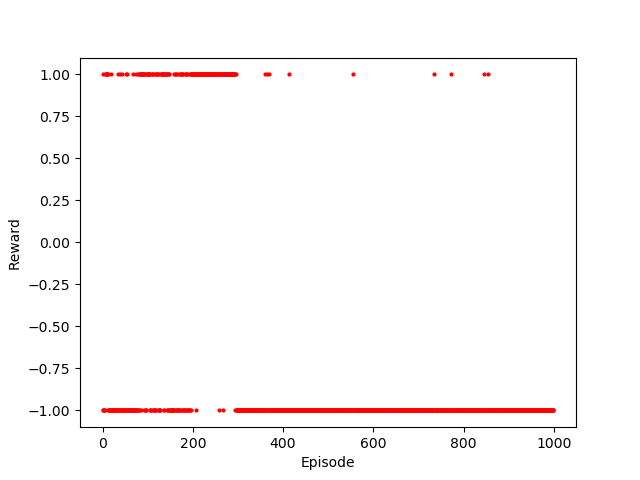
\includegraphics[width=6cm]{LeftiFFallreward_plot.png} }}%
    \qquad
    \subfloat[durchschnittlicher Reward]{{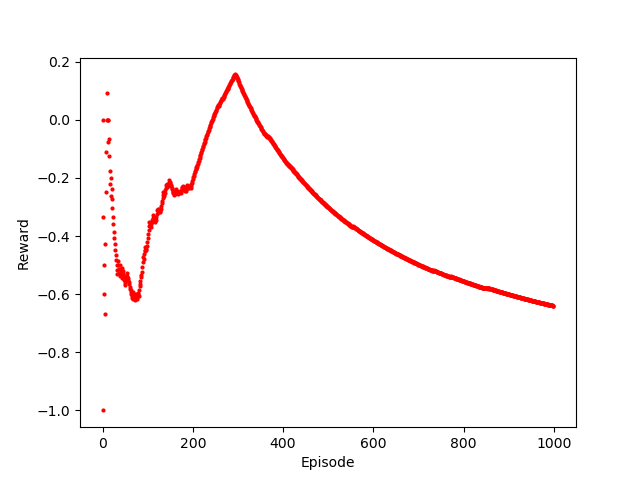
\includegraphics[width=6cm]{LeftiFFaveragereward_plot.png} }}%
    \caption{Reinforcement-Learning an deterministisch ziehendem Gegner mit einfacher Reward-Funktion und ohne die Züge des Gegners mitzulernen.}%
    \label{fig:leftiFF}%
\end{figure}

\begin{figure}%
    \centering
    \subfloat[absoluter Reward]{{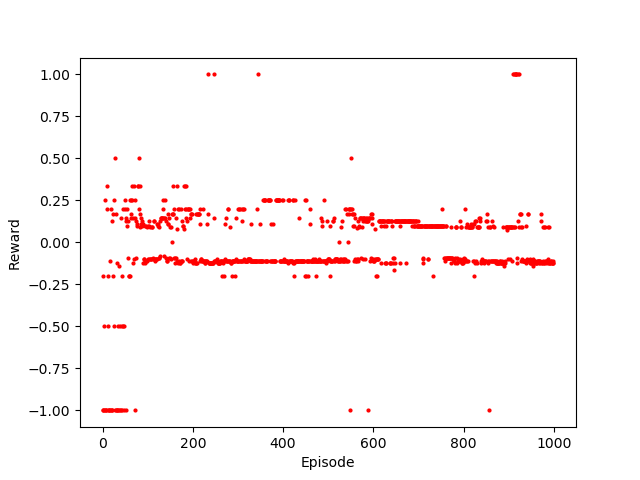
\includegraphics[width=6cm]{LeftiTFallreward_plot.png} }}%
    \qquad
    \subfloat[durchschnittlicher Reward]{{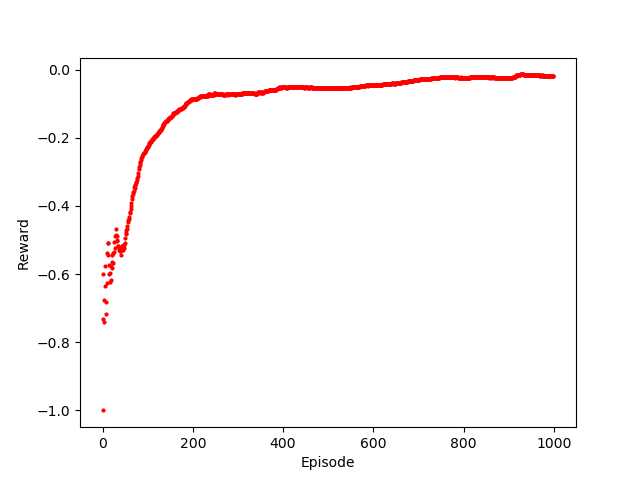
\includegraphics[width=6cm]{LeftiTFaveragereward_plot.png} }}%
    \caption{Reinforcement-Learning an deterministisch ziehendem Gegner mit verbesserter Reward-Funktion und ohne die Züge des Gegners mitzulernen.}%
    \label{fig:leftiTF}%
\end{figure}
Es wurde gezeigt, dass durch die zugabhängige Reward-Funktion besser gegen den zufälligen und den deterministischen Gegner gespielt wurde.
Hieraus schließe ich, dass die zugabhängige Reward-Funktion einen positiven Effekt auf das Lernverhalten des Reinforcement-Learning-Agenten hat.
Aus diesem Grund wird in allen fortlaufenden Evaluierungen mit der verbesserten Reward-Funktion gearbeitet.

\section{Lernen vom Gegner}
Nun wird evaluiert, ob das Lernen von den Zügen des Gegners einen positiven Einfluss auf das Lernverhalten des Agenten hat. Hierfür werden wieder der deterministisch und der zufällig ziehende Gegner genutzt.\\
Wie in Abbildung \ref{fig:randomTT} (b) zu sehen ist, ist das Ergebnis hier im Vergleich zu Abbildung \ref{fig:randomTF} (b) wesentlich schlechter. Dies ergibt aber Sinn, da der Gegner komplett zufällig spielt und somit das Lernen seiner Züge eher als Nachteil betrachtet werden muss.\\
Abbildung \ref{fig:leftiTT} zeigt hingegen eine sehr starke Verbesserung im Vergleich zu Abbildung \ref{fig:leftiTF}. Wie in Abbildung \ref{fig:leftiTT}(a) zu sehen ist, sind die meisten Rewards oberhalb von 0, dies war in Abbildung \ref{fig:leftiTF}(a) nicht der Fall.\\


\begin{figure}%
    \centering
    \subfloat[absoluter Reward]{{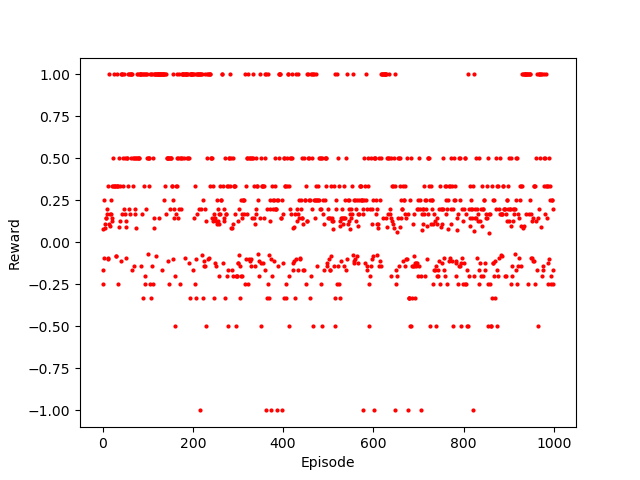
\includegraphics[width=6cm]{RandomTTallreward_plot.png} }}%
    \qquad
    \subfloat[durchschnittlicher Reward]{{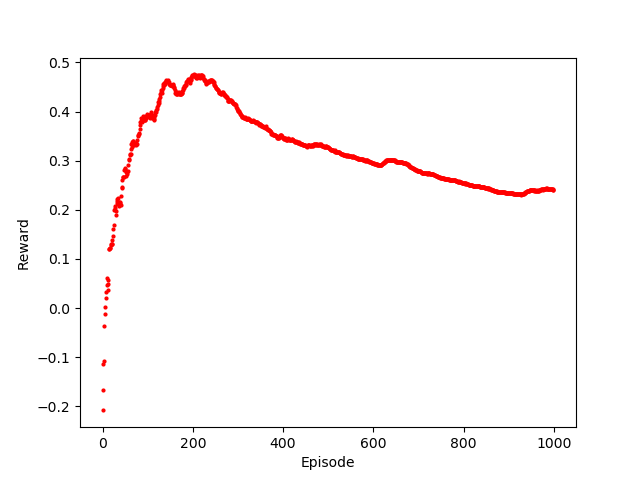
\includegraphics[width=6cm]{RandomTTaveragereward_plot.png} }}%
    \caption{Reinforcement-Learning an zufällig ziehendem Gegner mit verbesserter Reward-Funktion, wobei die Züge des Gegners mitgelernent werden.}%
    \label{fig:randomTT}%
\end{figure}

\begin{figure}%
    \centering
    \subfloat[absoluter Reward]{{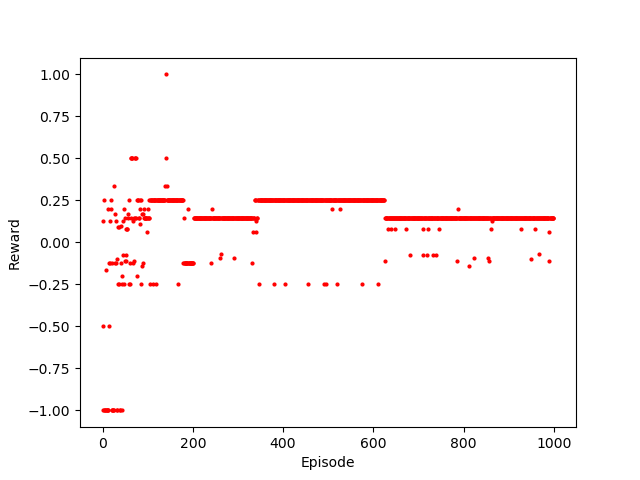
\includegraphics[width=6cm]{LeftiTTallreward_plot.png} }}%
    \qquad
    \subfloat[durchschnittlicher Reward]{{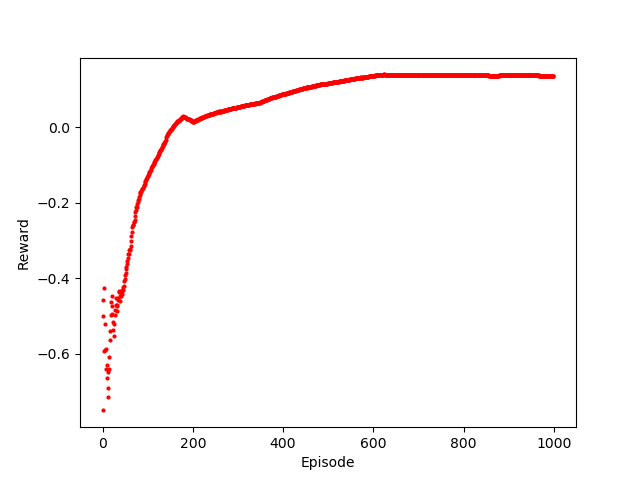
\includegraphics[width=6cm]{LeftiTTaveragereward_plot.png} }}%
    \caption{Reinforcement-Learning an zufällig ziehendem Gegner mit verbesserter Reward-Funktion, wobei die Züge des Gegners mitgelernent werden.}%
    \label{fig:leftiTT}%
\end{figure}

Somit wurde gezeigt, dass das Nutzen der Züge eines Gegners mit zielführender Strategie zu einer Verbesserung des Lernverhaltens des Reinforcement-Learning-Agenten führt.
Da in den folgenden Tests nur noch gegen Gegner mit einer zielführenden Strategie gelernt wird, wird das Lernen von gegnerischen Zügen für alle folgenden Evaluationen genutzt.

\section{Training am Gegner mit Minimax-Algorithmus}
Die letzte Evaluierung sollte zeigen, dass ein Reinforcement-Learning-Agent mit den zuvor gezeigten Verbesserungen unterschiedlich schnell zu einer guten Strategie finden kann. 
Hierfür wurde der Reinforcement-Learning-Agent gegen den Minimax-Algorithmus mit verschieden starker Wahrscheinlichkeitsverteilung trainiert.\\
Die in Abbildung \ref{fig:MiniMaxReward1} und Abbildung \ref{fig:MiniMaxReward2} gezeigten Graphen zeigen das Trainingsverhalten gegen den Minimax-Algorithmus. Diese sind nach steigender Wahrscheinlichkeit den besten Zug zu wählen geordnet. Das erste Paar in Abbildung \ref{fig:MiniMaxReward1} (a und b) hat somit die niedrigste Wahrscheinlichkeit den besten Zug zu wählen und das letzte Paar in Abbildung \ref{fig:MiniMaxReward2} (c und d) die höchste.\\
Leider ließ sich hier kein Lernfortschritt feststellen, nicht mal bei der niedrigsten Wahrscheinlichkeit. 

\begin{figure}%
    \centering
    \subfloat[absoluter Reward]{{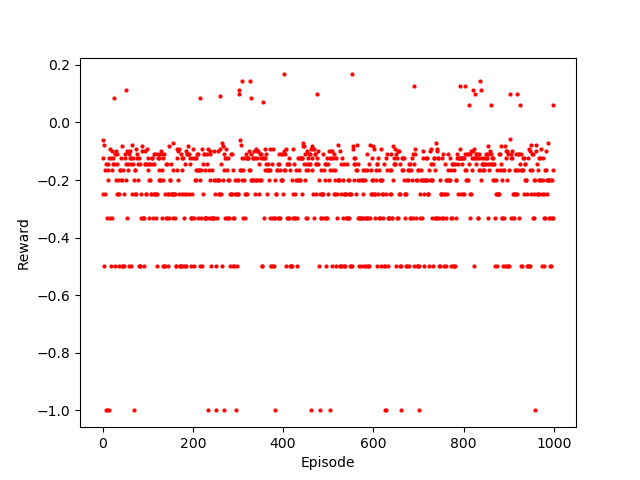
\includegraphics[width=6cm]{MM00001allreward_plot.png} }}%
    \qquad
    \subfloat[durchschnittlicher Reward]{{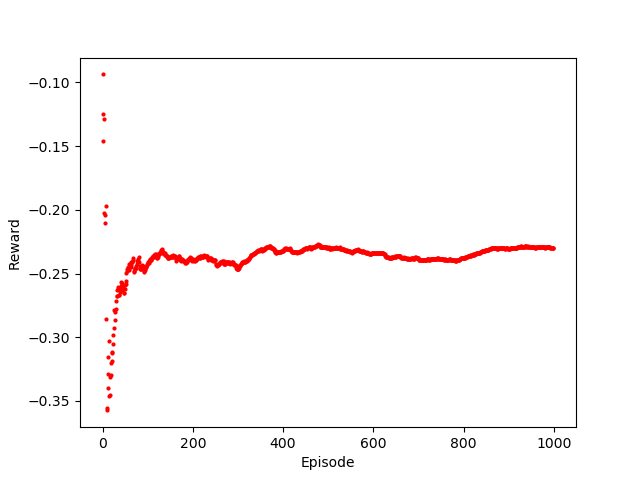
\includegraphics[width=6cm]{MM00001averagereward_plot.png} }}%
    \qquad
    \subfloat[absoluter Reward]{{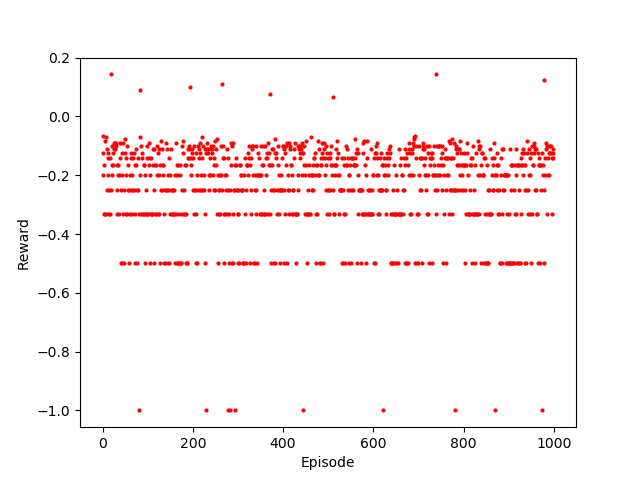
\includegraphics[width=6cm]{MM0001allreward_plot.png} }}%
    \qquad
    \subfloat[durchschnittlicher Reward]{{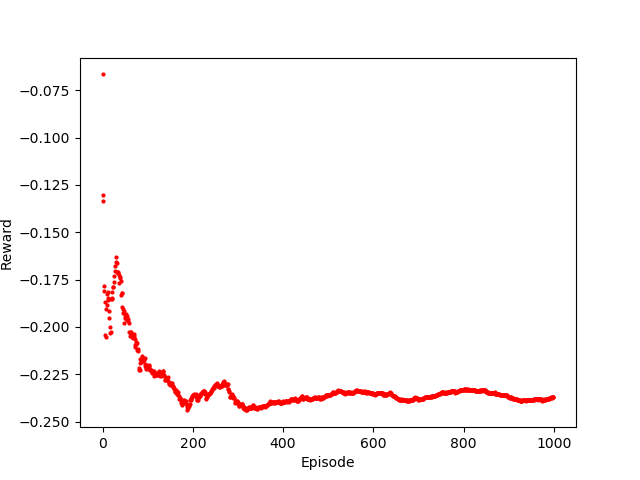
\includegraphics[width=6cm]{MM0001averagereward_plot.png} }}%
    \qquad
    \subfloat[absoluter Reward]{{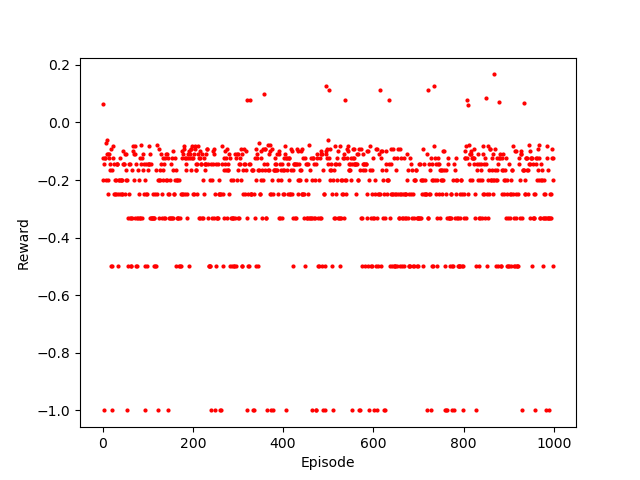
\includegraphics[width=6cm]{MM001allreward_plot.png} }}%
    \qquad
    \subfloat[durchschnittlicher Reward]{{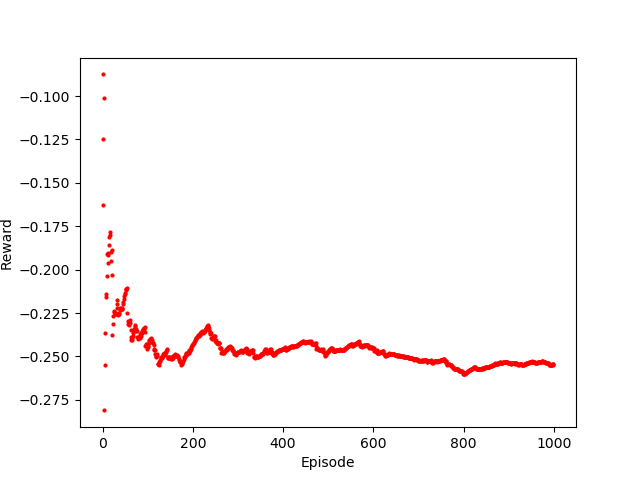
\includegraphics[width=6cm]{MM001averagereward_plot.png} }}%
    \qquad
    \subfloat[absoluter Reward]{{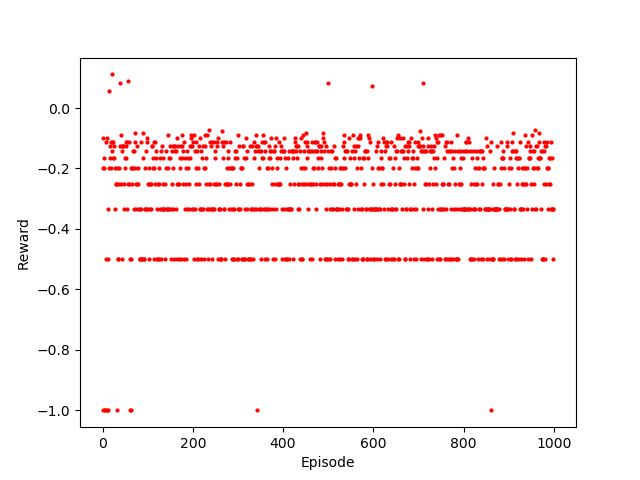
\includegraphics[width=6cm]{MM01allreward_plot.png} }}%
    \qquad
    \subfloat[durchschnittlicher Reward]{{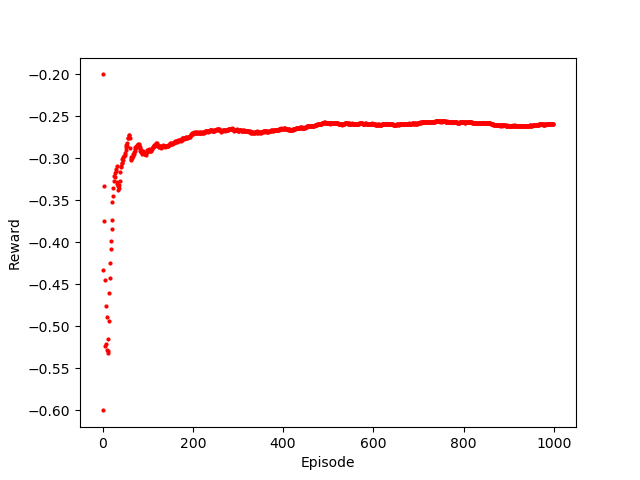
\includegraphics[width=6cm]{MM01averagereward_plot.png} }}%
    \caption{Reinforcement-Learning an Minimax Gegner mit verbesserter Reward-Funktion, wobei die Züge des Gegners mitgelernent werden. Teil 1}%
    \label{fig:MiniMaxReward1}%
\end{figure}
\begin{figure}%
    \centering
    \subfloat[absoluter Reward]{{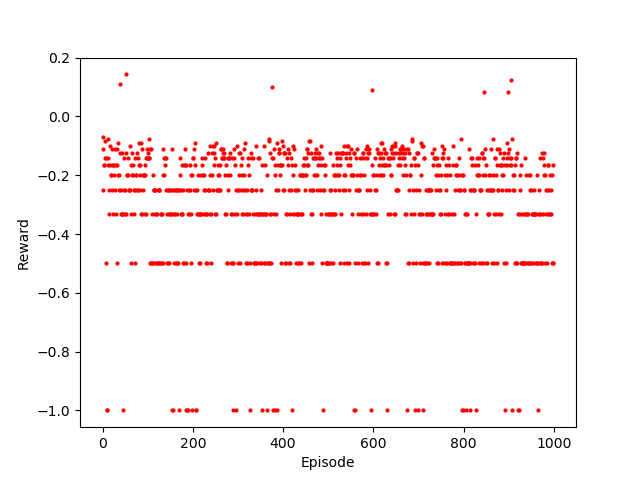
\includegraphics[width=6cm]{MM1allreward_plot.png} }}%
    \qquad
    \subfloat[durchschnittlicher Reward]{{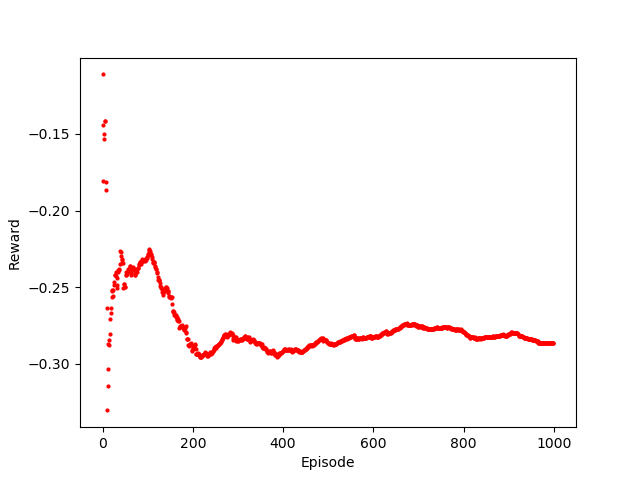
\includegraphics[width=6cm]{MM1averagereward_plot.png} }}%
    \qquad
    \subfloat[absoluter Reward]{{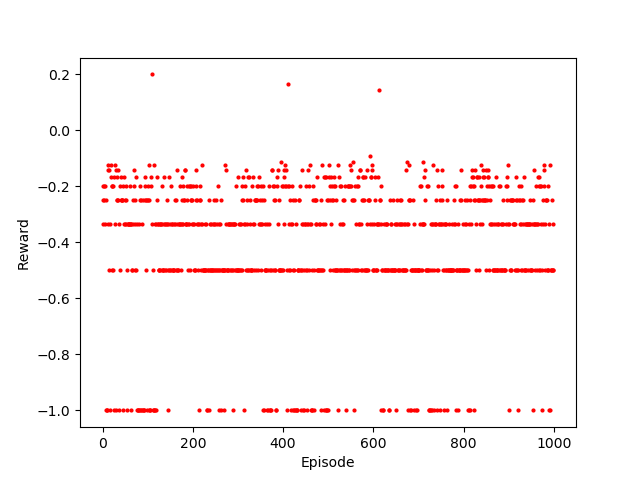
\includegraphics[width=6cm]{MM10allreward_plot.png} }}%
    \qquad
    \subfloat[durchschnittlicher Reward]{{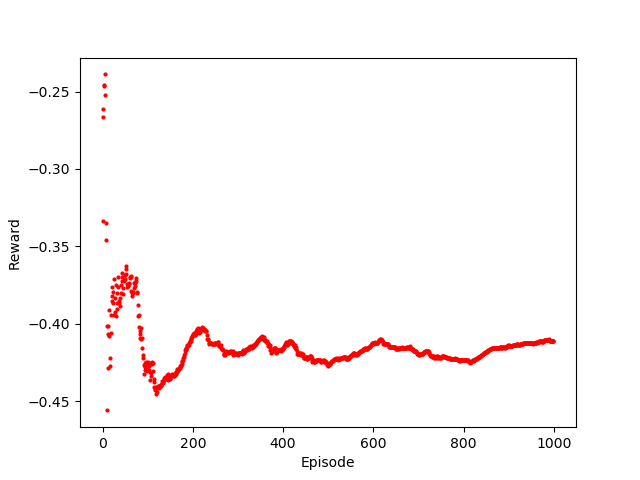
\includegraphics[width=6cm]{MM10averagereward_plot.png} }}%
    \caption{Reinforcement-Learning an Minimax Gegner mit verbesserter Reward-Funktion, wobei die Züge des Gegners mitgelernent werden. Teil 2}%
    \label{fig:MiniMaxReward2}%
\end{figure}

\section{Besonderheiten}
In den Graphen der Evaluation existiert eine Auffälligkeit, die bei ungefähr 250 bis 300 Episoden auftritt. Ist diese Anzahl an Episoden überschritten wird das Lernverhalten des Agenten oft schlagartig schlechter. Dies ist am deutlichsten in der Abbildung \ref{fig:leftiFF}(b) zu sehen. Ich vermute, dass dies mit der Epsilon-Greedy Policy zusammenhängt, die in dem Raum etwa den Maximalen Wert für $\epsilon$ erreicht hat.





